%\begin{figure}[h]
%    \centering
%	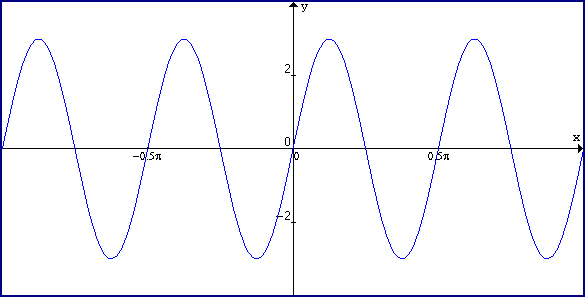
\includegraphics[scale=0.5]{graph}
%	\caption{An example graph}
%	\label{fig:x sine graph}
%\end{figure}


\newcommand{\doccount}{N}
\newcommand{\featcount}{V}
\newcommand{\streamlen}{T}
\newcommand{\traj}{y}
\newcommand{\df}{DF}
\newcommand{\featset}{\text{M}}

\newcommand{\docoverlap}{\text{d}}
\newcommand{\featsim}{\text{JSD}}

\newcommand{\bowmat}{\mat{B}}
\newcommand{\dtdmat}{\mat{D}}
\newcommand{\trajmat}{\mat{T}}


The core of this algorithm is taken from \cite{event-detection}.

\section{Document fetching}
We assume a collection of $N$ documents $\left\{ d_{1}, d_{2}, \dots, d_{\doccount} \right\}$ where for each document $d_{i}$, we know its publication day $t_{i}$. Then, the documents can be understood as a stream $\left\{ (d_{1}, t_{1}), (d_{2}, t_{2}), \dots, (d_{\doccount}, t_{\doccount}) \right\}$ with $t_{i} \leq t_{j}$ for $i < j$. Furthermore, we define $\streamlen$ to be the length of the stream, and we normalize the document publication days to be relative to the document stream start; that is $t_{1} = 1$ and $t_{\doccount} = \streamlen$.


\section{Bag of words model}
% TODO: blah blah we use the well known (binary) bag of words model, which drops the word order
To vectorize the documents, we define a matrix $\bowmat \in \left\{ 0, 1 \right\}^{\doccount \times \featcount}$, where $\featcount$ is the total vocabulary size. The document collection can then be interpreted as a set of $\doccount$ observations, each consisting of $\featcount$ binary features. The matrix $\bowmat$ is defined as

\begin{equation} \label{eq:bow-matrix}
	\bowmat_{ij} \coloneqq
	\begin{cases}
		1, & \text{document}~i~\text{contains the feature}~j \text{;} \\
		0, & \text{otherwise.}
	\end{cases}
\end{equation}

To limit the feature space, we trim the words appearing in less than 30 documents or in more than 90\% of the documents. The idea behind this is that the words appearing only in few documents cannot possibly represent relevant events, and are mostly anomalies. On the other hand, words appearing in most of the documents are likely stopwords, and do not carry much information. This helps to prune the feature space and makes $\bowmat$ reasonably sized.

From now on, we focus our analysis on the individual word features rather than whole documents.


\section{Computing feature trajectories}
The previous section represented word features in the document domain. This section focuses on representing these features in the time domain.

The time trajectory of a feature $f$ is a vector $\vect{\traj}_f = \left[ \traj_{f}(1), \traj_{f}(2), \dots, \traj_{f}(\streamlen) \right]$. Each element $\traj_{f}(t)$ represents the relative frequency of the feature $f$ at time $t$. This frequency is defined using the DFIDF score:

\begin{equation}
	\traj_{f}(t) \coloneqq \underbrace{\frac{\text{\df}_{f}(t)}{\text{\doccount}(t)}}_{\text{DF}} \times \underbrace{\log{\frac{\doccount}{\text{\df}_{f}}}}_{\text{IDF}},
\end{equation}

where $\text{\df}_{f}(t)$ is the number of documents published on day $t$ containing the feature $f$ (time-local document frequency), $\text{\doccount}(t)$ is the number of documents published on day $t$ and $\text{\df}_{f}$ is the number of documents containing the feature $f$ (global document frequency).

These feature trajectories are stored in a matrix $\trajmat \in \R^{\featcount \times \streamlen}$, with $\vect{\traj}_f$ being the $f$-th row of $\trajmat$. Here we take advantage of the normalization of the publication days, since they can now be used as column indices of $\trajmat$.

To make the computation efficient, we vectorize most of the operations. Along with the matrix $\bowmat$ defined in \ref{eq:bow-matrix}, we define a matrix $\dtdmat \in \left\{ 0, 1 \right\}^{\doccount \times \streamlen}$ mapping the documents to their publication days:

\begin{equation}
	\dtdmat_{ij} \coloneqq
	\begin{cases}
		1, & \text{document}~i~\text{was published on day}~j \text{;} \\
		0, & \text{otherwise}.
	\end{cases}
\end{equation}

Next, we sum the rows of $\bowmat$ together to obtain $\vect{\df} = \left[ \text{\df}_{1}, \text{\df}_{2}, \dots, \text{\df}_{\featcount} \right]$, and similarly the rows of $\dtdmat$ to obtain $\vect{\doccount}_{t} = \left[ \text{\doccount}(1), \text{\doccount}(2), \dots, \text{\doccount}(\streamlen) \right]$.

Using these matrices and vectors, we can compute $\trajmat$ as follows:

\begin{equation}
	\trajmat \coloneqq
		\underbrace{\text{diag} \left( \log{\frac{\doccount}{\vect{\df}}} \right)}_{\text{IDF}}
		\times
		\underbrace{\bowmat^{\T}
		\times \dtdmat
		\times \text{diag} \left( \frac{1}{\vect{\doccount}_{t}} \right)}_{\text{DF}}
\end{equation}


\section{Spectral analysis}
The next step is to employ spectral analysis techniques borrowed from signal processing to discover periodicities in the features. Results from this section are further used to categorize the word features.

We apply the discrete Fourier transform to each feature trajectory, yielding $\mathcal{F} \vect{\traj}_{f} = \left[ X_{1}, X_{2}, \dots, X_{\streamlen}\right ]$ such that

\begin{equation*}
	X_{k} = \sum_{t = 1}^{\streamlen}{\traj_{f}(t) \me^{- \frac{2 \pi \mi}{\streamlen} (k - 1) t}}, ~ k \in \{1, 2, \dots, \streamlen\}.
\end{equation*}

That way, we move from the time-domain of publication days to the frequency domain, where we can analyze how powerful each feature is. To do this, we need to estimate the power spectral density, which we do using the periodigram

\begin{equation*}
	\vect{P} = \left[ \|X_{1}\|^{2}, \|X_{2}\|^{2}, \dots, \|X_{\ceil{\streamlen / 2}}\|^{2} \right].
\end{equation*}

We define the dominant power spectrum of the feature $f$ as the maximum element of the periodogram, that is

\begin{equation}
	\text{DPS}_{f} \coloneqq \max_{k \leq \ceil{\streamlen / 2}}{\|X_{k}\|^{2}}.
\end{equation}

and the dominant period as the inverse of the frequency corresponding to the dominant power spectrum:

\begin{equation}
	\text{DP}_{f} \coloneqq \frac{1}{\mathit{freq}}.
\end{equation}

where \textit{freq} is the frequency corresponding to $\text{DPS}_{f}$.

When applied to rows of the matrix $\trajmat$, this method yields two vectors, $\vect{DPS} \in \R^{\featcount}$ and $\vect{DP} \in \N^{\featcount}$, containing the dominant power spectra and dominant periods, respectively.


\section{Feature categorization}
Based on the dominant power spectra and dominant periods, we divide the features into \underline{H}igh power-\underline{H}igh period and \underline{H}igh power-\underline{L}ow period categories \footnote{\cite{event-detection} actually define \textit{five} such categories; however, our method uses only the two sets of the most powerful features.}:

\begin{equation}
\begin{split}
	\mathit{HH} \coloneqq \left\{ f \mid \text{DPS}_{f} > \textit{dps-bound}, \text{DP}_{f} > \ceil{\streamlen / 2} \right\}, \\
	\mathit{HL} \coloneqq \left\{ f \mid \text{DPS}_{f} > \textit{dps-bound}, \text{DP}_{f} \leq \ceil{\streamlen / 2} \right\}.
\end{split}
\end{equation}

{\color{red}TODO: Define dps-bound!}


\section{Trajectory preprocessing}
During the event detection itself, we will need to measure the similarity of two trajectories. However, due to the general noisiness of the trajectories, the similarities are not computed directly. Most features would then seem far apart due to mild bursts malforming the trajectories, while not really contributing to the underlying events. Thus, the trajectories are first preprocessed.

\subsection{Burst filtering}
As we are only interested in the dominant bursts around the main events, we filter out the mild ones. We do this by computing a cutoff value for each feature trajectory and discarding all trajectory elements falling under this cutoff. This procedure is adopted from \cite{online-search-queries}. The algorithm is as follows:

\begin{algorithm}[H]
\begin{algorithmic}[1]
\caption{Burst filtering}
\Input $\text{window-length} ~ w$

\ForEach {$\vect{\traj}_{f} \in \{ \vect{\traj}_{1}, \vect{\traj}_{2}, \dots, \vect{\traj}_{\featcount}\}$}
	\State $\vect{MA}_{w} \gets \text{Moving Average of length} ~ w ~ \text{for} ~ \vect{\traj}_{f} = \left[ \traj_{f}(1), \traj_{f}(2), \dots, \traj_{f}(\streamlen) \right]$

	\State $\mathit{cutoff} \gets \text{mean} \left( \vect{MA}_{w} \right) + \text{std} \left( \vect{MA}_{w} \right)$

	\State $\vect{bursts}_{f} \gets \left[ \traj_{f}(t) \mid \traj_{f}(t) > \mathit{cutoff}, \traj_{f}(t) \in \vect{y}_{f} \right]$
\EndFor

\Output $\{ \vect{bursts}_{1}, \vect{bursts}_{2}, \dots, \vect{bursts}_{\featcount} \}$

\end{algorithmic}
\end{algorithm}

{\color{red} TODO: In the paper, they use $\vect{MA}(t)_{w} > \mathit{cutoff}$, try that. Also, why did I miss that? :(}

\subsection{Normalization}
From now on, we assume the individual trajectories have been normalized to have unit sums. This can be computed efficiently by vectorizing the operation and dividing every row of $\trajmat$ by its sum. Thanks to this normalization, the individual trajectories can be interpreted as probability distributions over the stream days.

\subsection{Smoothing}

\begin{enumerate}

\item \textbf{Aperiodic features}

\textbf{TODO}

\item \textbf{Periodic features}

\textbf{TODO}

\end{enumerate}


\section{Event detection}

During the event detection phase, the aim is to find sets of features highly correlated both in the time domain and in the document domain. The assumption is that features appearing in similar documents during the same time periods concern the same real-world events. Each such feature set then represents a single event.

By inspecting only the sets of high power features, we uncover only the features best describing the individual events. This also helps to reduce computation time, since there are generally much fewer high power features than the low power ones.

The aperiodic and periodic features are detected separately, since we assume no connection between aperiodic events and the periodic ones.


\subsection{Measuring trajectory similarity}

Similarity between two feature trajectories is defined in terms of their information divergence. Unlike \cite{event-detection}, we use the \textit{Jensen-Shannon} divergence:

\begin{equation*}
	\featsim \left( \vect{p} \| \vect{q} \right) = \frac{1}{2} \text{D} \left( \vect{p} \| \vect{m} \right) + \frac{1}{2} \text{D} \left( \vect{q} \| \vect{m} \right),
\end{equation*}

where $\vect{m} = \frac{1}{2} \left( \vect{p} + \vect{q} \right)$ and D denotes the \textit{Kullback-Leibler} divergence.

The JS-divergence is symmetric, and its square root is a proper metric. It can also be computed without using the \textit{max} function, unlike the approach chosen by \cite{event-detection}, which makes the computation somewhat faster.

This similarity is then generalized to a set of features $\featset$ as

\begin{equation}
	\featsim \left( \featset \right) = \max{ \{ \featsim ( \vect{y}_{f_{i}} \| \vect{y}_{f_{j}} ) \mid f_{i}, f_{j} \in \featset \} }
\end{equation}

{\color{red}TODO: Use the JSD formula for multiple distributions?}


\subsection{Measuring document overlap}

The document overlap is first defined for two features, and then generalized to a whole feature set.

Let $\featset_{i}$ be the set of all documents containing a feature $f_{i}$, and $\featset_{j}$ the set of all documents containing a feature $f_{j}$. Then, the document overlap of the features $f_{i}$ and $f_{j}$ is defined as

\begin{equation}
	\docoverlap(f_{i}, f_{j}) \coloneqq \frac{\left\vert{\featset_{i} \cap \featset_{j}}\right\vert}{\min \left( {\left\vert{\featset_{i}}\right\vert, \left\vert{\featset_{j}}\right\vert} \right)}.
\end{equation}

Using this definition, the document overlap of a set of features $\featset$ can be defined as

\begin{equation}
	\docoverlap \left( \featset \right) \coloneqq \min{\{ \docoverlap \left( f_{i}, f_{j} \right) \mid f_{i}, f_{j} \in \featset \}}.
\end{equation}

Since we aim to maximize the document overlap among a set of features, it makes sense to define it using minimum, as it takes care of the worst possible case.


\subsection{Event detection}

\textbf{TODO}